\section{哈密顿图}
\begin{definition}
%@see: 《离散数学》(邓辉文) P194 定义7-2
设\(G = (V,E)\)是图.
\begin{itemize}
	\item \(G\)中经过所有顶点一次且仅一次的路径,
	称为\DefineConcept{哈密顿路径}(Hamiltonian path).

	\item \(G\)中经过所有顶点一次且仅一次(除起点重复一次外)的圈,
	称为\DefineConcept{哈密顿回路}(Hamiltonian cycle)
	或\DefineConcept{哈密顿环}%
	或\DefineConcept{哈密顿圈}.

	\item 存在哈密顿回路的图,
	称为\DefineConcept{哈密顿图}(Hamiltonian graph).
\end{itemize}
\end{definition}

显然,由哈密顿回路可以得到哈密顿路径,不返回出发点即可,
但是,反过来一般不成立.
在\cref{figure:图论.哈密顿路径1} 中,存在哈密顿路径\(bcaed\),但不存在哈密顿回路.
在\cref{figure:图论.哈密顿图1} 中,存在哈密顿回路\(v_1 v_5 v_4 v_3 v_2 v_1\),它是哈密顿图.

\begin{figure}[hbt]
%@see: 《离散数学》(邓辉文) P194 图7-8(a)
	\centering
	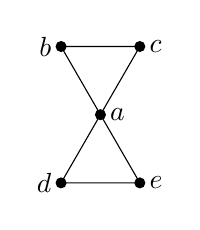
\begin{tikzpicture}
		\fill(0,0)coordinate(a)node[right]{$a$}circle(2pt);
		\fill(-.5,{.5*sqrt(3)})coordinate(b)node[left]{$b$}circle(2pt);
		\fill(.5,{.5*sqrt(3)})coordinate(c)node[right]{$c$}circle(2pt);
		\fill(-.5,{-.5*sqrt(3)})coordinate(d)node[left]{$d$}circle(2pt);
		\fill(.5,{-.5*sqrt(3)})coordinate(e)node[right]{$e$}circle(2pt);
		\draw(a)--(b)--(c)--(d)--(e)--(a);
	\end{tikzpicture}
	\caption{}
	\label{figure:图论.哈密顿路径1}
\end{figure}

\begin{figure}[hbt]
%@see: 《离散数学》(邓辉文) P194 图7-8(b)
	\centering
	\def\n{5}
	\def\b{90}
	\begin{tikzpicture}
		\pgfmathsetmacro{\m}{\n-1}
		\pgfmathsetmacro{\a}{360/\n}
		\foreach \j in {0,...,\m} {
			\fill({cos(\j*\a+\b)},{sin(\j*\a+\b)})coordinate(A\j)circle(2pt);
		}
		\draw(A0)node[above]{$v_1$}
			(A1)node[left]{$v_2$}
			(A2)node[below]{$v_3$}
			(A3)node[below]{$v_4$}
			(A4)node[right]{$v_5$};
		\begin{scope}[-{Latex[length=3mm,width=0pt 10]}]
			\draw(A0)--(A2);
			\draw(A0)--(A3);
			\draw(A0)--(A4);
			\draw(A1)--(A0);
			\draw(A2)--(A1);
			\draw(A2)--(A4);
			\draw(A3)--(A2);
			\draw(A3)--(A1);
			\draw(A4)--(A3);
			\draw(A4)--(A1);
		\end{scope}
	\end{tikzpicture}
	\caption{}
	\label{figure:图论.哈密顿图1}
\end{figure}

显然,
一个无向哈密顿图是连通图,
一个有向哈密顿图是强连通图.

\begin{theorem}
%@see: 《离散数学》(邓辉文) P195 定理7-5
设\(G = (V,E)\)是无向哈密顿图,
则\[
	(\forall W)
	[
		\emptyset \neq W \subset V
		\implies
		w(G-W) \leq \abs{W}
	].
\]
%TODO proof
\end{theorem}

\begin{example}
%@see: 《离散数学》(邓辉文) P195 例7-3
举例说明:无向图\(G = (V,E)\)满足\[
	(\forall W)
	[
		\emptyset \neq W \subset V
		\implies
		w(G-W) \leq \abs{W}
	],
\]
但不是哈密顿图.
%TODO 彼得森图
\end{example}

1960年,Ore得到一个哈密顿图的充分条件.
\begin{theorem}
%@see: 《离散数学》(邓辉文) P195 定理7-6(Ore,1960)
设\(G = (V,E)\)是\(n\ (n\geq3)\)阶简单无向图.
若\[
	(\forall u,v \in V)
	\left[
		\text{$u$与$v$不邻接}
		\implies
		\deg u + \deg v \geq n
	\right],
\]
则\(G\)是哈密顿图.
%TODO proof
\end{theorem}

\begin{example}
%@see: 《离散数学》(邓辉文) P196 例7-4
举例说明:\(n\ (n\geq3)\)阶简单无向图\(G = (V,E)\)不满足\[
	(\forall u,v \in V)
	\left[
		\text{$u$与$v$不邻接}
		\implies
		\deg u + \deg v \geq n
	\right],
\]
但它是哈密顿图.
%TODO
\end{example}

Ore的上述成果推广了Dirac于1952年给出的结果.
\begin{corollary}
%@see: 《离散数学》(邓辉文) P196 推论(Dirac,1952)
设\(G = (V,E)\)是\(n\ (n\geq3)\)阶简单无向图.
若\[
	(\forall v \in V)
	[\deg v \geq n/2],
\]
则\(G\)是哈密顿图.
%TODO proof
\end{corollary}

\begin{theorem}
%@see: 《离散数学》(邓辉文) P196 定理7-7
设\(G = (V,E)\)是\(n\ (n\geq3)\)阶无向图.
若\[
	(\forall u,v \in V)
	\left[
		\text{$u$与$v$不邻接}
		\implies
		\deg u + \deg v \geq n-1
	\right],
\]
则\(G\)中存在哈密顿路径.
%TODO proof
\end{theorem}

\begin{example}
%@see: 《离散数学》(邓辉文) P196 例7-5
设\(G = (V,E)\)是\(n\ (n\geq3)\)阶连通无向图.
证明:\(G\)中存在两个顶点\(u,v\),
将它们删除后得到的图\(G-\{u,v\}\)仍是连通的.
%TODO proof
\end{example}

%TODO
% 旅行商问题(travelling salesman problem)/货郎担问题
% 假设有\(n\)个城镇,其中任意两个城镇之间都有道路.
% 一个售货员要去这\(n\)个城镇售货,
% 从某城镇出发,依次访问其余\(n-1\)个城镇,
% 且每个城镇只能访问一次,最后又回到原出发地.
% 问售货员要如何安排经过\(n\)个城镇的旅行路线,
% 才能使他经过的路程最短.
% 该问题的本质是,在一个边赋权图中,找出一条权最小的哈密顿回路.
% 这是一个比判断一个图是否哈密顿图更困难的的问题.
% 当然,如果给定的赋权图是一个3阶以上的完全无向图,则哈密顿回路的存在性是显然的.
% 要求解这个问题,可以先将所有哈密顿回路找出来,再比较它们的权的大小,求出权最小的哈密顿回路即可.
% 但是对于阶数较大的赋权图来说,这样做的计算量太大.
% 求旅行商问题的近似解有“近似法”和“交换法”.
% 除此以外,人们还在研究利用遗传算法、模拟退货算法、神经网络、蚁群算法以及粒子群算法等算法.
